
Bilingual and multilingual psycholinguistics corpora have been used to evaluate the psychometric fit of language models beyond English \citep{de-varda-marelli-2023-scaling, wilcox2023language, xu2023linearity}. The Multilingual Eye-movement Corpus (MECO), a multilingual corpus of eye tracking data collected on simple Wikipedia-style articles, originally collected for 13 languages \cite{siegelman2022expanding} building on earlier bilingual corpora such as Ghent Eye-Tracking Corpus (GECO; \citealp{colman-etal-2022-geco}), which focused on Dutch–English bilingual sentence reading within a more limited linguistic scope. MECO has recently been extended to 20 languages \cite{siegelman2025wave}. MECO enables controlled comparisons of reading behaviour across languages and within individuals reading in both L1 and L2. In contrast, other L2 eye tracking datasets (e.g., CELER \cite{berzak2022celer}) prioritise typological diversity in L1 learners in L2 English but lack the cross-lingual comparability of MECO. 

\paragraph{MECO Eye Tracking Dataset.} We test whether token-level surprisal across the \beetle{} bilingual model family predicts L2 English reading times from the Multilingual Eye-Movement Corpus  MECO Wave 1 and 2 Eye Tracking Data of L2 learners of English \citep{siegelman2022expanding, kuperman2023text,siegelman2025wave,kuperman2025new}.\footnote{\url{https://meco-read.com/}} MECO~L2 provides population-scale eye-tracking data for L2 English readers for typologically diverse L1s, letting us analyse how exposure structure interacts with reader-L1 distance from English.  

\paragraph{Method.}  We use \beetle{} to model L2 first-pass reading time (gaze duration) in the MECO eye-tracking dataset\citep{siegelman2022expanding, kuperman2023text, siegelman2025wave, kuperman2025new}, matching model and human L1s. We predict word reading time using linear mixed-effects regression models, including the word's (and two preceding words') LM surprisal, length, and position in the document as fixed effects, and random intercepts and slopes for all subjects. For each target word $w_i$ we compute LM surprisal $S(w_i) = -\log P(w_i \mid w_{<i})$ from every \beetle{} checkpoint and every baseline. We fit a mixed-effects regression of first-pass (first-run) duration (\texttt{firstrun.dur}) on current and spillover surprisal with word-level controls (length, \texttt{wordfreq} log-frequency, sentence position) and by-subject random intercepts plus random slopes on surprisal (full specification in Eq.~\ref{eq:meco-spec}, App.~\ref{sec:meco-results}). Following \citet{wilcox-etal-2023-language}, the psychometric predictive-power score is $\Delta\log L = \log L(\mathrm{full}) - \log L(\mathrm{baseline})$, where the baseline drops the three surprisal terms. Since raw $\Delta\log L$ scales with sample size, we standardise within each reader-L1 group, reporting effects in within-language SD units \citep{de-varda-marelli-2022-effects}. To probe stage-specific alignment, we additionally interact surprisal with the MECO reading-time measure (first-pass / first-run duration = early lexical access; refixations = intermediate; regressions-in = late integration; \citealp{siegelman2025wave}). With only eight language clusters, we use OLS with language fixed effects and a wild-cluster bootstrap clustered by language (Rademacher weights, $B=4999$; \citealp{cameron2008bootstrap}), and apply Benjamini--Hochberg FDR correction across contrasts.

\subsection{Key result: curriculum beats scale on MECO~L2}\label{sec:reading-time-headline}


%Reading-time alignment is the canonical psycholinguistic readout for an LM \citep{wilcox2020predictive, wilcox-etal-2023-language}; the closest L2 prior is \citet{de-varda-marelli-2022-effects}, who use mBERT pseudo-surprisal on MECO~L2 and report a substantial L2 attenuation gap relative to L1 reading. \beetle{} differs in two ways. First, we treat exposure curricula (not parameter scale, \citealp{de-varda-marelli-2023-scaling}) as the primary axis of variation. Second, we report first-pass (first-run) duration, gaze duration, and total reading time separately to test whether the L1 early/late dissociation also holds for L2.

Surprisal estimates from matched \beetle{} models significantly predict MECO~L2 reading times across L1-reader groups in MECO. We analyse \beetle{} MECO results at (i) averages across the full \beetle{} model family, (ii) the strongest individual models within the \beetle{} family, and (iii) comparisons against external multilingual and bilingual LLM baselines.  Across \beetle{} 125M parameter models, the \beetle{} family consistently outperforms a comparison pool of modern bilingual and multilingual LLMs on every released reader-L1 condition. For Dutch~L2 readers, the mean \beetle{} score reaches $\Delta\log L = \mathbf{81.10}$, compared with 12.04 for the comparator aggregate. For German~L2 readers, the corresponding values are $\mathbf{167.04}$ versus 90.85, while for Chinese~L2 readers they are $\mathbf{130.41}$ versus 55.71.\footnote{The comparator aggregate is the arithmetic mean across XGLM-4.5B, EuroLLM-1.7B, EuroLLM-9B, Apertus-8B, Gemma-2-9B, Qwen-3-8B, and Llama-3.1-8B; full per-model results are reported in Tab.~\ref{tab:meco_baseline_comparators}.} The average \beetle{} advantage is approximately $6.7\times$ on Dutch~L2, $1.8\times$ on German~L2, and $2.3\times$ on Chinese~L2. \citet{de-varda-marelli-2022-effects} report that LMs tend to predict L2 reading times worse for second language speakers. \beetle{} models do not show this L2 attention effect. Compared to  multilingual LLMs, \beetle models effectively eliminate any attenuation effects, particularly for German (the strongest matched model is B2 deu--eng FW, which reaches $\Delta\log L = 184.7$ on the German-reader condition), or at least substantially reduce it (e.g., Dutch result is obtained by B3-33 nld--eng HS attains a mean score of $\overline{\Delta\log L}=170.0$)


Beetle MECO model and per-comparator breakdowns appear in App.~\ref{sec:meco-results}; bootstrap forest, mixed-effects diagnostics, item-level surprisal grids, and per-participant breakdowns appear in App.~\ref{appcomp:meco}.


\subsubsection{Effect of \beetle{} Exposure Curricula}

We observe consistent benefits of “staged” curricula (L2 curricula, B2 - B5) over balanced bilingual B1, with roughly 50 MECO~$\Delta\log L$ lower performance (Fig.~\ref{fig:bA8_typology_per_curriculum} for the per-curriculum typological profile across L1s). 

 The within-\beetle{} curriculum effect attenuates monotonically with L1--English typological distance, with the Germanic L1s (nld, deu) carrying the strongest curriculum spread and the Chinese L1s substantially compressed (Fig.~\ref{fig:meco_curriculum};)
 

\subsubsection{\beetle{}-L2LM and LLM Comparison} \label{sec:comparator-landscape}

The cleanest controlled comparison is provided by the simultaneous nl--en B-GPT model of \citet{arnett-etal-2025-acquisition}, since both systems are 125M-parameter Dutch--English bilinguals trained under broadly similar curriculum assumptions. On the matched Dutch-reader MECO condition, B-GPT achieves $\Delta\log L = 88.25$, whereas \beetle{} B3-33 nld--eng HS reaches $\mathbf{139.6}$, corresponding to a $\mathbf{1.58\times}$ improvement. Unlike the BLOOM comparisons, this evaluation avoids major parameter-scale and corpus-composition confounds and therefore constitutes the clearest curriculum-controlled baseline comparison in the paper. On the cross-L1 German- and Chinese-reader conditions, however, B-GPT slightly exceeds \beetle{} (243.0 / 221.6 versus \beetle{}'s 222.8$^{\dagger}$ / 184.8 respectively). 

\paragraph{\beetle{} v LLMs} From a token efficiency perspective, structured-exposure pretraining in \beetle{} models surpasses MECO performance threshold achieved by BLOOM-7b1 while using only a fraction of its training budget, and the advantage associated with the B3-33 and B5 curricula continues to increase with additional training. We interpret this pattern as suggestive of a bilingual analogue to the monolingual $\sim$2B-token tipping point identified by \citet{aoyama-wilcox-2025-language}, potentially arising earlier under structured bilingual exposure. On the matched Dutch-reader MECO condition, B3-33 nld--eng HS ($139.6$) substantially outperforms every checkpoint in the BLOOM family. Relative to \textbf{BLOOM-560m} ($44.29$), which has approximately 4.5$\times$ as many parameters as \beetle{}, the gain is $3.15\times$. Relative to the much larger \textbf{BLOOM-7b1} ($19.69$; roughly 56$\times$ the parameter count), the gain increases to $7.1\times$. The Dutch-reader BLOOM mean is 32.83, yielding an overall advantage of approximately $4.25\times$. These comparisons remain confounded by differences in tokenizer design and training-corpus composition (ROOTS versus FineWeb/BabyBabelLM), so they do not isolate curriculum effects directly. Rather, they demonstrate that scale alone does not recover the curriculum-controlled advantage observed for matched-data \beetle{} models. On Chinese~L2, by contrast, the BLOOM ladder mean (131.65) exceeds the strongest HumanScale \beetle{} Chinese model, B5 zho--eng HS (115.4), with BLOOM-1b1 reaching 164.3. We discuss this typological boundary case further in \S\ref{sec:limitations-control}.

Comparison with a broader multilingual LLM cohort --- including XGLM-4.5B, EuroLLM-1.7B/9B, Apertus-8B, Gemma-2, Qwen-3, and Llama-3.1-8B --- shows \beetle{} provides substantially better performance on the matched Dutch- and German-reader conditions. The Chinese-reader condition presents a more mixed picture: the European multilingual models remain below \beetle{}'s strongest HumanScale Chinese result (115.4), whereas the Japanese-focused LLM-JP-3 variants exceed it, consistent with their substantially greater Chinese-corpus exposure. 


See Tab.~\ref{tab:meco_full_canonical} and \S\ref{sec:reading-time-headline}



\begin{figure*}[!ht]
\centering
    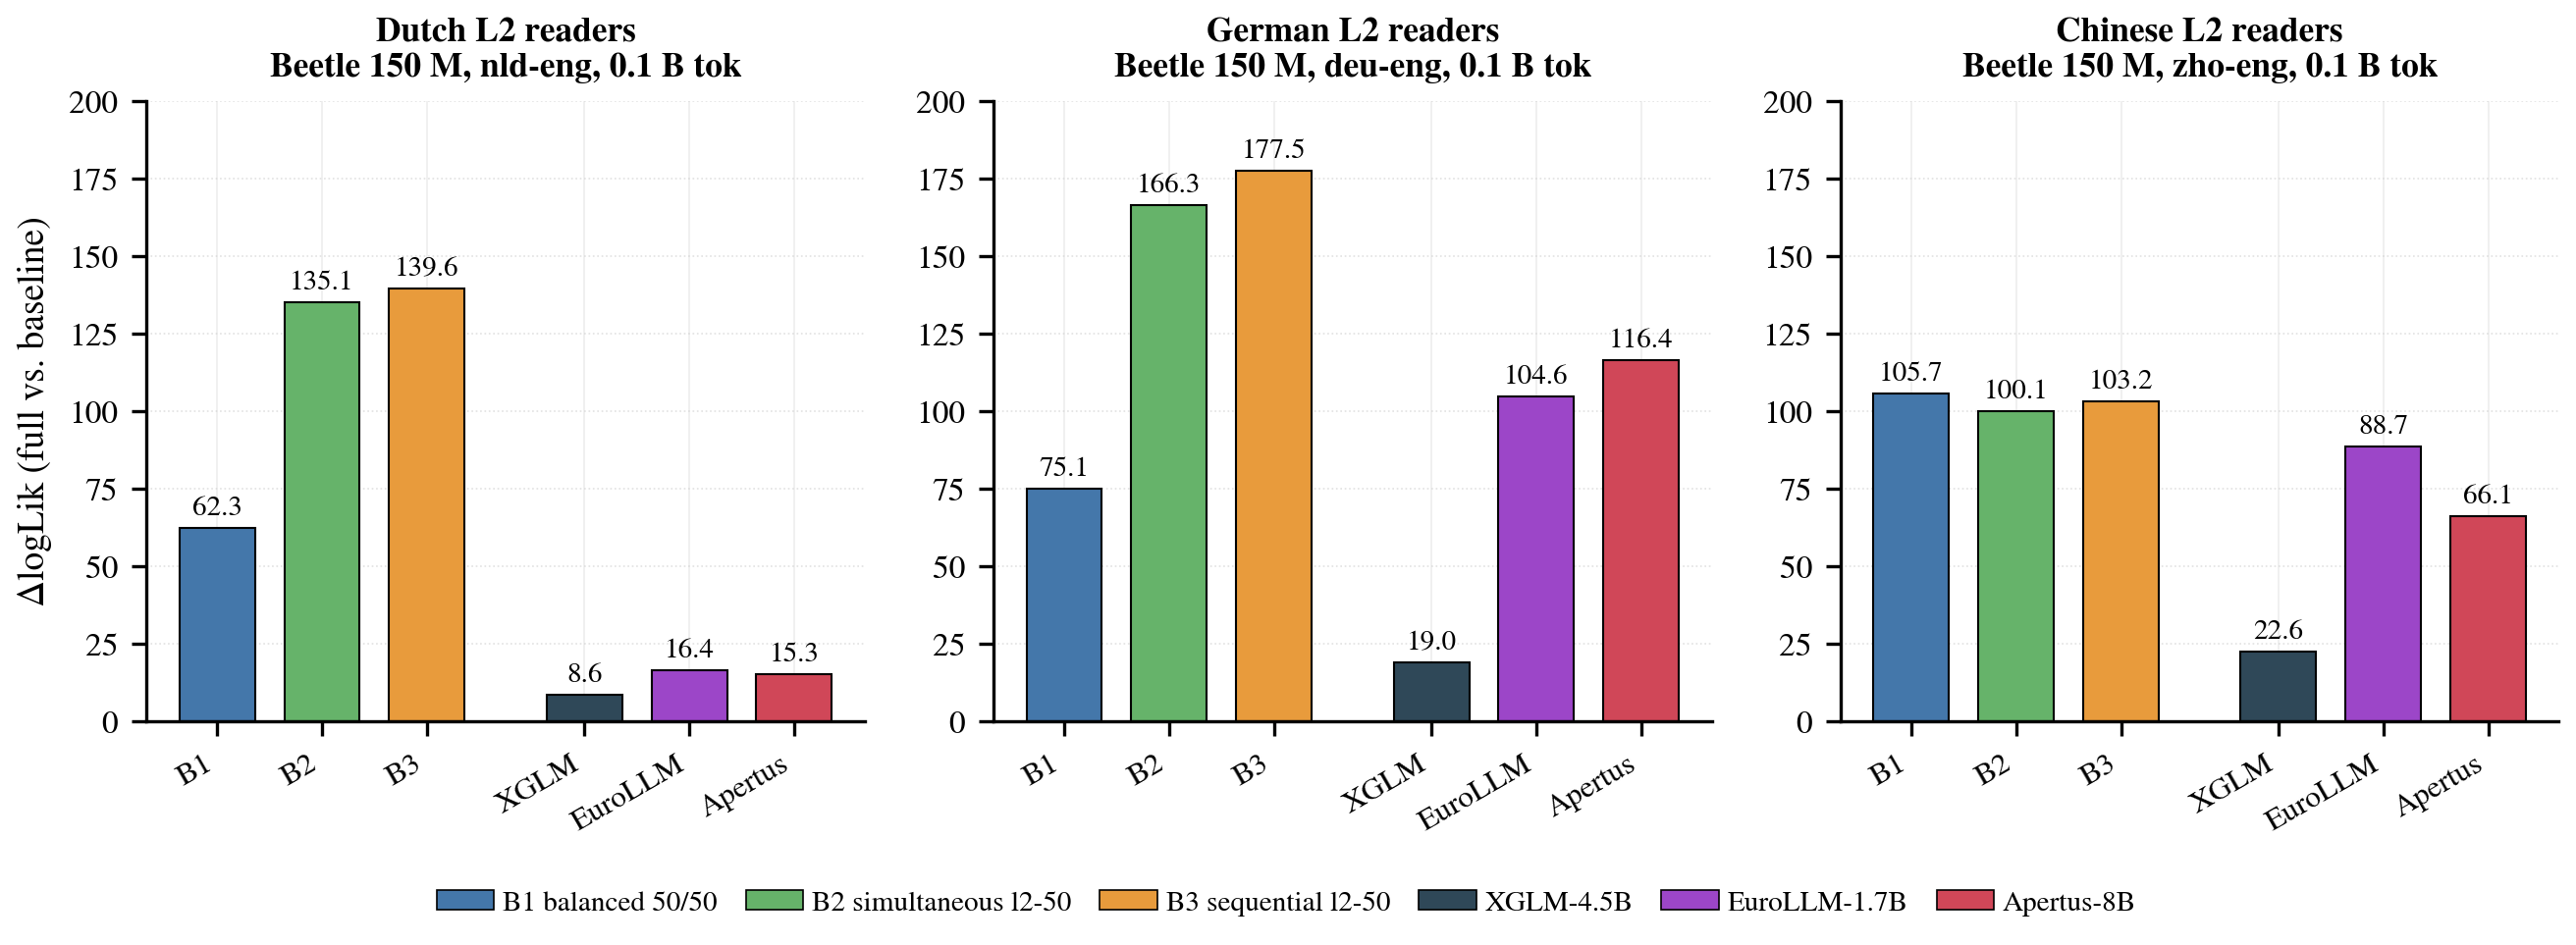
\includegraphics[width=\linewidth]{fig/meco/F4_curriculum_meco_deltaLL_baselines.png}
    \caption{\small{Evaluation of \textsc{Beetle} models with balanced bilingual (B1) and sequential second language exposure (B2, B3, differing in proportion of L1:L2) conditions on English L2 MECO with L1 Dutch (nld), German (deu), and Chinese (zho) MECO participants\citep{siegelman2022expanding,siegelman2025wave}. $\Delta$logLik is the improvement in regression log-likelihood over a baseline regression excluding surprisal predictors. We see that compared to larger multilingual LMs, \textsc{Beetle} LMs achieve consistently higher alignment with MECO reading time, with a clear additional impact of exposure schedule for the Dutch-English and German-English \textsc{Beetle} LMs.}}
    \label{fig:meco_curriculum}
\end{figure*}

%\begin{figure*}[!ht]
%  \centering
%  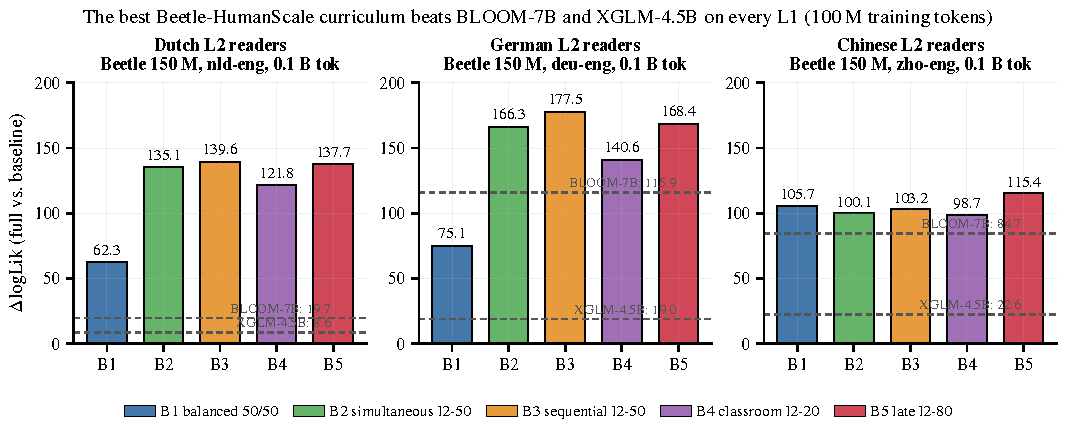
\includegraphics[width=\linewidth]{fig/meco/F4_curriculum_meco_deltaLL.pdf}
%  \caption{\textbf{Within-\beetle{} curriculum advantage.} MECO~L2 $\Delta\log L$ by exposure curriculum (B1 balanced, B2 simultaneous, B3-33 sequential, B4 classroom, B5 late onset) for Dutch (\textsc{nld}), German (\textsc{deu}), and Chinese (\textsc{zho}) L2 reader groups. Higher $\Delta\log L$ indicates stronger reading-time alignment. Sequential B3-33 and late-onset B5 dominate matched-L1 Germanic cells (B3-33 nld--eng HS = 139.6 on the matched Dutch-reader cell; B2 deu--eng FW = 184.7 on the matched German-reader cell). On Chinese L2 the matched-L1 effect holds within HumanScale (B5 zho--eng HS = 115.4); the cross-class comparator picture against BLOOM and the modern bilingual LLMs is reported separately in \S\ref{sec:comparator-landscape}.}
%  \label{fig:meco_curriculum}
%\end{figure*}

%Surprisal from matched \beetle{} models predicts MECO~L2 reading times in the three released reader-L1 groups (Dutch, German, Chinese) with significant coefficients, extending \citet{de-varda-marelli-2022-effects} (Germanic L1s only) beyond Germanic to a Sino-Tibetan reader cohort; the remaining five reader-L1 groups (spa, rus, fin, tur, heb) are corpus-prepared and queued (App.~\ref{sec:roadmap} item~1).

%At the \emph{group level} --- averaging across all 33 \beetle{} 125M bilinguals at HumanScale and FineWeb --- \beetle{} leads on every reader-L1: $\Delta\log L = $ \textbf{81.10} for Dutch L2, \textbf{167.04} for German L2, and 130.41 for Chinese L2, against a seven-model modern bilingual / multilingual LLM aggregate\footnote{The seven aggregated models are XGLM-4.5B, EuroLLM-1.7B, EuroLLM-9B, Apertus-8B, Gemma-2-9B, Qwen-3-8B, and Llama-3.1-8B (arithmetic mean across the seven rows of Tab.~\ref{tab:meco_baseline_comparators}); full per-model breakdown in the same table.} of 12.04 / 90.85 / 55.71 on Dutch / German / Chinese L2 respectively. The group-level advantage is $6.7\times$ on Dutch, $1.8\times$ on German, and $2.3\times$ on Chinese.

%At the \emph{within-\beetle{} single-model level}, the best \beetle{} is B3-33 nld--eng HS with matched Dutch-reader $\Delta\log L = \textbf{139.6}$ (the 3-reader-group mean $\overline{\Delta\log L} = 170.0$ is inflated by the cross-L1 German cell flagged with a dagger in Tab.~\ref{tab:meco_full_canonical}; we do not read that cell as load-bearing). B2 deu--eng FW reaches 184.7 on the matched German-reader cell. The L2 attenuation gap of \citet{de-varda-marelli-2022-effects} is closed for German~L2 and substantially narrowed for Dutch~L2.

%\emph{\beetle v BGPT \citep{arnett-etal-2025-acquisition}}   B-GPT nl--en simultaneous \citep{arnett-etal-2025-acquisition}: same 125M parameter class, same nl--en language pair, similar curriculum philosophy. On the same matched Dutch-reader MECO cell, B-GPT reaches $\Delta\log L = 88.25$; \beetle{} B3-33 nld--eng HS exceeds it by $\mathbf{1.58\times}$. This is the cleanest curriculum-controlled comparison we have, because the data-composition confound that affects the BLOOM ratios (\S\ref{sec:comparator-landscape}) is absent: both are nl--en bilinguals at 125M. On the cross-L1 German- and Chinese-reader cells, by contrast, B-GPT slightly leads (243.0 vs.~Beetle's matched-L1 best 177.5; 221.6 vs.~115.4 on matched Chinese L2 HS); we treat the cross-L1 cells as part of the comparator-landscape picture rather than as headline claims (\S\ref{sec:comparator-landscape}).

\begin{figure}[!ht]
  \centering
  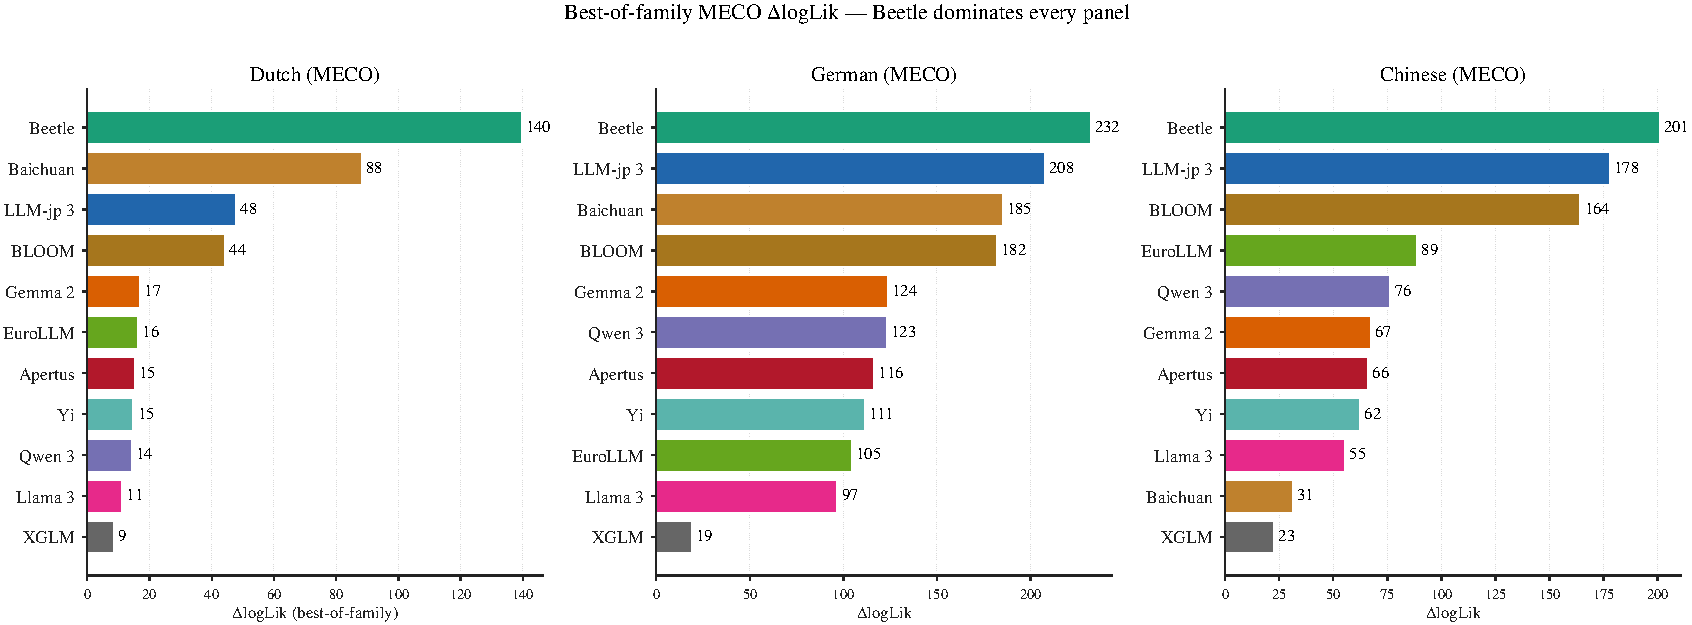
\includegraphics[width=\linewidth]{fig/fig_meco_best_of_family.pdf}
  \caption{MECO~L2 $\Delta\log L$ as a function of training tokens for \beetle{} curricula (B1--B5; nld--eng, deu--eng) against the BLOOM ladder and XGLM-4.5B. Sequential B3-33 and late B5 cross the BLOOM-7b1 threshold before 200M tokens and plateau above it.}
  \label{fig:meco_efficiency}
\end{figure}

%Fig.~\ref{fig:meco_efficiency} resolves the token-efficiency dimension: structured-exposure \beetle{} models exceed the BLOOM-7b1 MECO threshold at a fraction of its training budget, and the B3-33 / B5 advantage compounds with further training. We read this token-efficiency pattern as suggestive of a bilingual analogue to the monolingual $\sim$2\,B tipping point of \citet{aoyama-wilcox-2025-language} sitting earlier in training under structured exposure, while leaving the actual induction-head onset measurement to follow-up work (App.~\ref{sec:roadmap}).



%\paragraph{Within-\beetle{} curriculum-by-task synthesis}\label{sec:pareto}



\paragraph{\beetle{} v LLMs}

On the matched MECO~L2 Dutch-reader cell, B3-33 nld--eng HS (139.6) exceeds the smallest BLOOM checkpoint, \textbf{BLOOM-560m} (44.29; $\sim$4.5$\times$ Beetle's parameter count), by $3.15\times$, and exceeds the much-larger \textbf{BLOOM-7b1} (19.69; 56$\times$ params) by $7.1\times$. The BLOOM ladder mean on Dutch is 32.83 (4.25$\times$ gap).

\paragraph{\beetle{} v BLOOM.}  These ratios are confounded with data composition (ROOTS vs.\ FineWeb / BabyBabelLM) and tokeniser, so they show that scale alone does not lift the legacy ladder to the matched-data curriculum-controlled \beetle{} cell, but do not isolate the curriculum effect. On Chinese L2, by contrast, the BLOOM ladder mean (131.65) leads B5 zho--eng HS (115.40); BLOOM-1b1 specifically reaches 164.3 vs.\ Beetle's HumanScale best 115.4. We discuss this typological boundary in Limitations \S\ref{sec:limitations-control}.

\paragraph{Modern bilingual / multilingual LLM cohort.} The European-multilingual cohort (XGLM-4.5B, EuroLLM-1.7B / 9B, Apertus-8B, Gemma-2 2B / 9B, Qwen-3-4B / 8B, Llama-3.1-8B) trails \beetle{} substantially on the matched Dutch- and German-reader cells, while on the Chinese-reader cell the picture is mixed (European cohort below \beetle{}'s HumanScale best of 115.4; Japanese-multilingual LLM-JP-3 variants above it, consistent with their Chinese-corpus exposure). A cross-L1 transfer observation --- that at FineWeb scale Dutch-conditioned \beetle{} bilinguals score higher on Chinese readers than several European-multilingual baselines --- is reported in Tab.~\ref{tab:meco_full_canonical} as observational and not load-bearing on the within-\beetle{} curriculum claim.

\paragraph{Matched-architecture matched-language-pair prior (B-GPT).} The closest curriculum-controlled comparator is B-GPT nl--en simultaneous \citep{arnett-etal-2025-acquisition}: same 125M parameter class, same nl--en language pair, similar curriculum philosophy. \beetle{} B3-33 nld--eng HS reaches 1.58$\times$ B-GPT's matched-Dutch-reader $\Delta\log L$ (139.6 vs.\ 88.25; both single-seed point estimates). This is the cleanest curriculum-vs-prior-work comparator the paper has. On the cross-L1 German- and Chinese-reader cells, by contrast, B-GPT slightly leads (243.0 / 221.6 vs.\ Beetle's 222.8$^{\dagger}$ / 184.8, where the dagger marks the same single-seed German-reader cell flagged at); we report these for completeness and treat them as part of the cross-L1 transfer observation flagged for seed-grid replication.

\paragraph{Caveats.} (i) Headline cells are single-seed (\S\ref{sec:limitations-control}); within-\beetle{} curriculum differences will be more seed-sensitive than the across-class gaps. (ii) The 3.15$\times$ / 7.1$\times$ BLOOM ratios change comparator-by-comparator and \emph{are not used as the headline of the paper}; the curriculum-controlled 1.58$\times$ vs.\ B-GPT and the within-\beetle{} curriculum-by-task map (\S\ref{sec:pareto}) are.